%% 
%% Copyright 2007, 2008, 2009 Elsevier Ltd
%% 
%% This file is part of the 'Elsarticle Bundle'.
%% ---------------------------------------------
%% 
%% It may be distributed under the conditions of the LaTeX Project Public
%% License, either version 1.2 of this license or (at your option) any
%% later version.  The latest version of this license is in
%%    http://www.latex-project.org/lppl.txt
%% and version 1.2 or later is part of all distributions of LaTeX
%% version 1999/12/01 or later.
%% 
%% The list of all files belonging to the 'Elsarticle Bundle' is
%% given in the file `manifest.txt'.
%% 

%% Template article for Elsevier's document class `elsarticle'
%% with numbered style bibliographic references
%% SP 2008/03/01

\documentclass[preprint,12pt]{elsarticle}

%% Use the option review to obtain double line spacing
%% \documentclass[authoryear,preprint,review,12pt]{elsarticle}

%% Use the options 1p,twocolumn; 3p; 3p,twocolumn; 5p; or 5p,twocolumn
%% for a journal layout:
%% \documentclass[final,1p,times]{elsarticle}
%% \documentclass[final,1p,times,twocolumn]{elsarticle}
%% \documentclass[final,3p,times]{elsarticle}
%% \documentclass[final,3p,times,twocolumn]{elsarticle}
%% \documentclass[final,5p,times]{elsarticle}
%% \documentclass[final,5p,times,twocolumn]{elsarticle}

%% For including figures, graphicx.sty has been loaded in
%% elsarticle.cls. If you prefer to use the old commands
%% please give \usepackage{epsfig}

%% The amssymb package provides various useful mathematical symbols
\usepackage{amssymb}
\usepackage{algorithm}
\usepackage[noend]{algpseudocode}
\usepackage{algcompatible}

%% The amsthm package provides extended theorem environments
%% \usepackage{amsthm}

%% The lineno packages adds line numbers. Start line numbering with
%% \begin{linenumbers}, end it with \end{linenumbers}. Or switch it on
%% for the whole article with \linenumbers.
%% \usepackage{lineno}

\journal{Nuclear Physics B}

\begin{document}

\begin{frontmatter}

%% Title, authors and addresses

%% use the tnoteref command within \title for footnotes;
%% use the tnotetext command for theassociated footnote;
%% use the fnref command within \author or \address for footnotes;
%% use the fntext command for theassociated footnote;
%% use the corref command within \author for corresponding author footnotes;
%% use the cortext command for theassociated footnote;
%% use the ead command for the email address,
%% and the form \ead[url] for the home page:
%% \title{Title\tnoteref{label1}}
%% \tnotetext[label1]{}
%% \author{Name\corref{cor1}\fnref{label2}}
%% \ead{email address}
%% \ead[url]{home page}
%% \fntext[label2]{}
%% \cortext[cor1]{}
%% \address{Address\fnref{label3}}
%% \fntext[label3]{}

\title{Reducing Power Consumption in Huffman Coding}

%% use optional labels to link authors explicitly to addresses:
%% \author[label1,label2]{}
%% \address[label1]{}
%% \address[label2]{}

\author{}

\address{}

\begin{abstract}
%% Text of abstract

\end{abstract}

\begin{keyword}
%% keywords here, in the form: keyword \sep keyword

%% PACS codes here, in the form: \PACS code \sep code

%% MSC codes here, in the form: \MSC code \sep code
%% or \MSC[2008] code \sep code (2000 is the default)

\end{keyword}

\end{frontmatter}

%% \linenumbers

%% main text
\section{Introduction}
\section{Background}
\subsection{Huffman Coding}
\subsection{Power consumption}
\subsection{Issues in Biological data transmission}
\section{GA-SO : Genetic algorithm for Switches Optimising}
Genetic algorithm (GA) is one the of the most popular bio-inspired meta-heuristic algorithm inspired from the natural evolution of species []. It is a  population based algorithm starts with the generation of a random initial population. The population contain a set of feasible solutions called individuals, that are usually far from the optimal. The GA optimisation process uses a set of natural genetic operators such as selection, crossover and mutation to converge to the optimal solution.
\subsection{Preparing data and population generation}
Huffman algorithm read the whole message to compute frequencies. The proposed algorithm read the whole genome to generate the frequencies of the triplet and by the way to generate the adjacent matrix which represents the frequencies precedence of between triplet. The initial population is generated randomly, each solution on the population represents a tree that generates a set of codes equal to the total triplets number.
\subsection{Selection}
The first operator of the genetic algorithm is the selection []. The main objective of the selection is to choose the part of the current  population to be a candidate for the different genetic operators in order to breed the next generation population. Many selection techniques have been proposed in the literature []. In this approach the  process of natural selection is maintained. First we generate a random pair numbers \textit{$rand$} between 2 and the population size, this number represent how many parents will be processed. After that, an unbiased random selection of \textit{$rand$}~individuals (solutions) from the population is maid. 
\subsection{Crossover}
The main operator of the GA is the crossover, allows to construct new solutions from the selected part of the population. The selected solutions are ranked by fitness and crossover two by two from high fitness to low. The main objective of the crossover is to benefits from the two good solutions in order to generate a better solution. An internal node for each tree (solution) is selected (\textit{$node1$},\textit{$node2$}), these two nodes must have the same number of leaf nodes (contain the same number of codes). The crossover operation will create two new trees (solutions), the first child (second) contain the nodes that are not children of the \textit{$node1$} (\textit{$node2$}) and we replace the children of \textit{$node1$} (\textit{$node2$}) by the children of \textit{$node2$} (\textit{$node1$}) (see fig.1). 
\subsection{Mutation}
The mutation operator changes the positions of two leaf nodes of the generated children (result of the crossover); this introduce the diversity in the search process, this diversification strategy allow the algorithm do conference to the global optimum. The algorithm for this operator goes through the leaf nodes and change the position of two leaf nodes from a parent to another and selects the ones to change according to a fixed mutation rate (see fig.1).
\subsection{Population update}
The crossover operation aims to generate new solutions from the current solution to built the second generation of the population. Furthermore, the mutation provide the diversity on the search space solution by changing the position of  nodes on the same tree. After these two operations, the next step of the genetic algorithm is two to breed the new population. Firstly the new solutions (children) are added to the current population, after that the population is ranked by fitness. The algorithm remove the worst solutions until the initial size of the population is achieved. The algorithm genetic repeat these operators until the stopped criteria is achieved, in this algorithm the stopped criteria is when the objective function (number of switches) stop decreasing.
\begin{algorithm}[!btph]
\caption{Switches optimising Huffman codes}
\label{alg1}
\begin{algorithmic}[1]
\REQUIRE Textual representation of a Genome
\ENSURE Low switches Huffman codes
\STATE Generate triplet frequencies and adjacent matrix 
\STATE Generate the initial  population of trees
\REPEAT 
\STATE Select part of the population
\STATE Generate children candidates via crossover
\STATE Mutate children
\STATE Add children to population
\STATE Rank by fitness
\STATE Remove worst solutions until population limit
\UNTIL{The switches number stop decreasing}
%\algstore{myalg}
\end{algorithmic}
\end{algorithm}
\begin{figure}[t]
\begin{center}
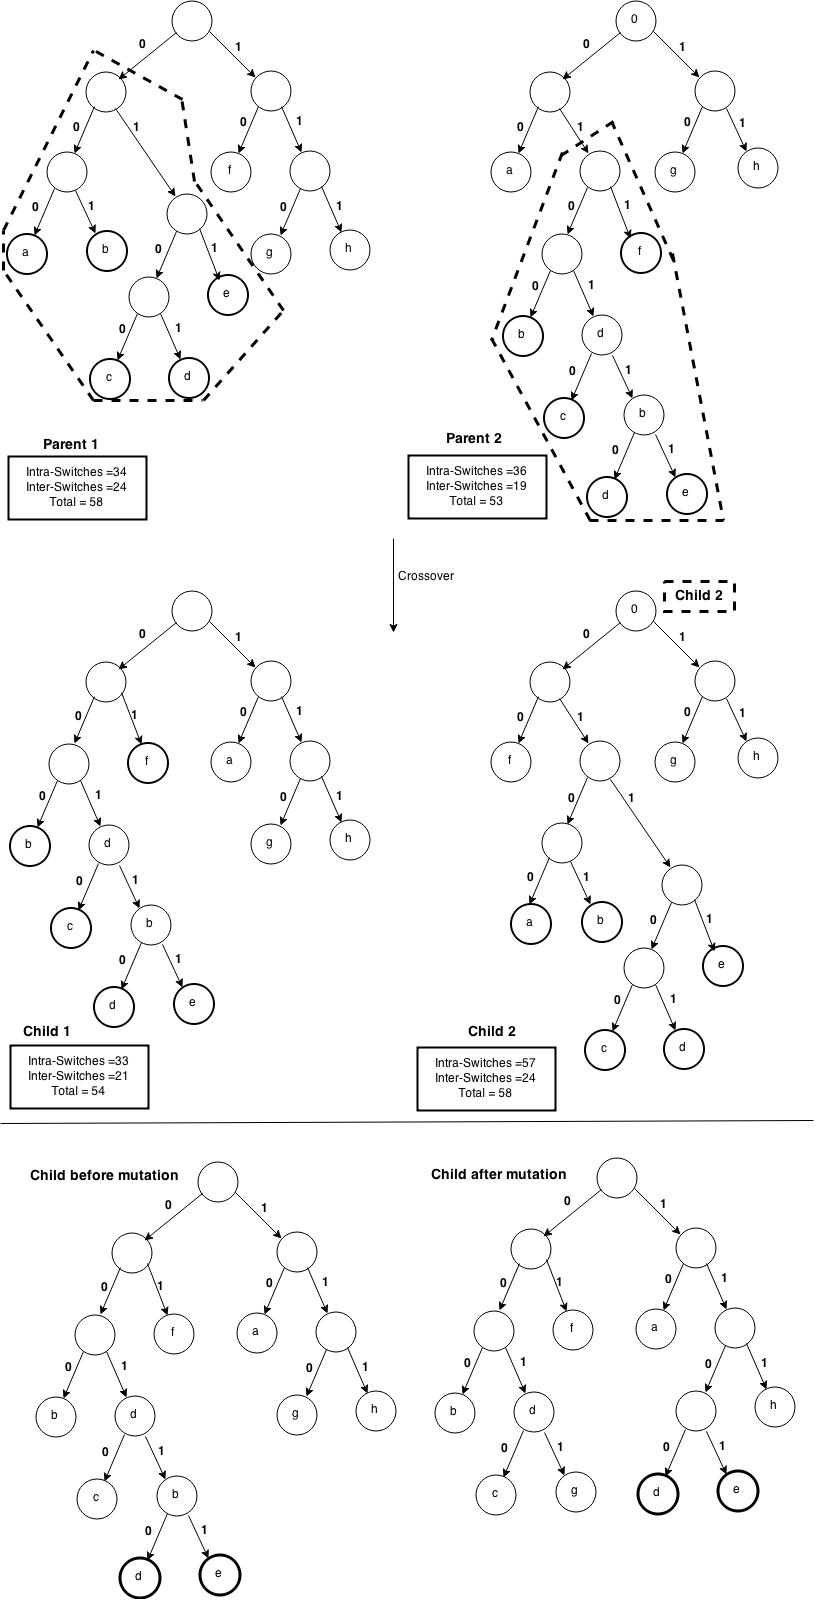
\includegraphics[width=400pt,height=545pt]{Images/Drawing1-1.jpg}
\caption{The Crossover operator}
\end{center}
\label{Fig1}
\end{figure}
\begin{figure}[h]
\begin{center}
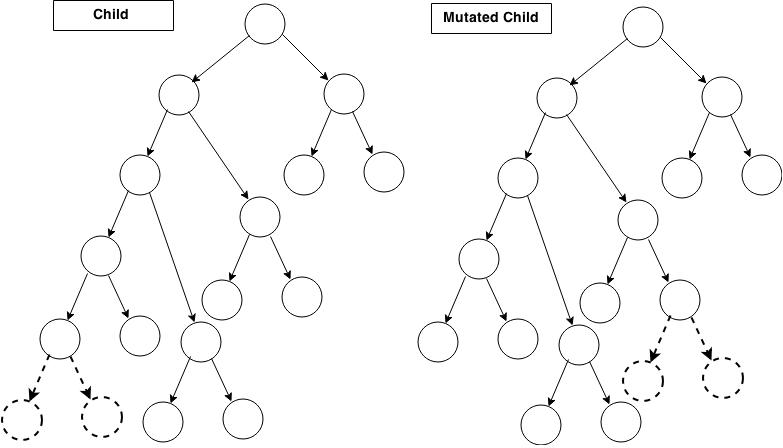
\includegraphics[width=200pt,height=200pt]{Images/Drawing2.jpg}
\caption{The Mutation operator}
\end{center}
\label{Fig1}
\end{figure}
\section{Experiments and Comparison}
\subsection{Datasets Description}
\subsection{Results}
\begin{table}[h]
\renewcommand{\arraystretch}{1.1}
\small
\label{table4}
\caption{Comparison of performance among classical Huffman code, CCA, and OCCA without penalty}
%\begin{center}

\begin{tabular}{c  c c  c c  c c}
\hline
 & Huffman Algorithm & P \\\hline
\\\hline
Genome 1& 18.16 & 10.05 & 44.65 \\\hline
Genome 2& 24.66 &  15.63 & 36.61 \\\hline
Genome 3&18.46 &  10.66&  42.25\\\hline
Genome 4&25.18&16.26& 35.42\\\hline
Genome 5& 19.24& 16.08 &16.42 \\\hline
Genome 6& 19.61&14.96&23.71\\\hline
Genome 7& 22.40 &13.21&41.02\\\hline
Genome 8&23.87 & \\\hline
Genome 9& &\\\hline
Genome 10& & \\\hline
Genome 11& & \\\hline
Genome 12& &\\\hline
Genome 13& &\\\hline
Genome 14& & \\\hline
Genome 15& & \\\hline
Genome 16&& \\\hline
Genome 17& & \\\hline
Genome 18& & \\\hline

%\bottomrule
\end{tabular}
%\end{center}
\end{table}
\section{Conclusion}

%% The Appendices part is started with the command \appendix;
%% appendix sections are then done as normal sections
%% \appendix

%% \section{}
%% \label{}

%% If you have bibdatabase file and want bibtex to generate the
%% bibitems, please use
%%
%%  \bibliographystyle{elsarticle-num} 
%%  \bibliography{<your bibdatabase>}

%% else use the following coding to input the bibitems directly in the
%% TeX file.

\begin{thebibliography}{00}

%% \bibitem{label}
%% Text of bibliographic item

\bibitem{}

\end{thebibliography}
\end{document}
\endinput
%%
%% End of file `elsarticle-template-num.tex'.
